\documentclass[11pt,a4paper]{article}
\usepackage[utf8]{inputenc}
\usepackage[margin=1in]{geometry}
\usepackage{amsmath,amssymb,amsfonts}
\usepackage{graphicx}
\usepackage{booktabs}
\usepackage{hyperref}
\usepackage{float}
\usepackage{caption}
\usepackage{subcaption}
\usepackage{cite}

\hypersetup{
    colorlinks=true,
    linkcolor=blue,
    filecolor=magenta,      
    urlcolor=cyan,
    pdftitle={Medical Image Captioning using CNN-LSTM Architecture},
}

\title{\textbf{Medical Image Captioning using CNN-LSTM Neural Networks: System Design, Empirical Evaluation, and Benchmark Comparison on ROCO v2}}
\author{\textbf{ROCO v2 Deep Learning Workspace Pipeline} \\
Department of Artificial Intelligence \& Deep Learning \\
\texttt{CNN+LSTM Project Repository}}
\date{August 2026}

\begin{document}

\maketitle

\begin{abstract}
Automated caption generation for medical imaging bridges the gap between computer vision and clinical text generation. This report provides a complete theoretical, architectural, and empirical analysis of a Deep Convolutional Neural Network (CNN) combined with a Long Short-Term Memory (LSTM) recurrent neural network for medical image captioning. The architecture utilizes a pretrained \textbf{ResNet-50} feature extractor coupled via a 512-dimensional linear projection to a single-layer \textbf{LSTM} sequence decoder. The system was trained on \textbf{59,958 radiology images} from the ROCO v2 dataset, validated on \textbf{9,904 images}, and evaluated on an independent test set of \textbf{9,927 images}. Empirical evaluation yields a final test Cross-Entropy Loss of \textbf{3.4785}, \textbf{BLEU-1} of \textbf{0.2105}, \textbf{BLEU-2} of \textbf{0.1098}, \textbf{BLEU-3} of \textbf{0.0624}, \textbf{BLEU-4} of \textbf{0.0377}, \textbf{METEOR} of \textbf{0.1721}, and \textbf{ROUGE-L} of \textbf{0.1953}. Furthermore, a comprehensive comparative study is conducted against the benchmark paper \textit{``Image Captioning Generator Using CNN and LSTM''} (IJRASET, June 2022), analyzing architectural differences, domain complexity (general open-domain vs. specialized radiology domain), and metric variance.
\end{abstract}

\section{Introduction \& System Architecture}

Medical image captioning requires generating cohesive natural language descriptions from high-dimensional visual inputs (e.g., CT scans, MRIs, and X-rays). The system architecture employs an encoder-decoder design where a Convolutional Neural Network (CNN) extracts visual features and a Recurrent Neural Network (LSTM) generates tokens autoregressively.

\subsection{CNN Feature Encoder}
Given an input image $I \in \mathbb{R}^{3 \times 224 \times 224}$, normalized using ImageNet statistics ($\boldsymbol{\mu} = [0.485, 0.456, 0.406]$, $\boldsymbol{\sigma} = [0.229, 0.224, 0.225]$), the ResNet-50 backbone $\phi_{\text{ResNet}}(\cdot)$ extracts a global visual representation:
\begin{equation}
\mathbf{f}_{\text{raw}} = \text{AvgPool}(\phi_{\text{ResNet}}(I)) \in \mathbb{R}^{2048}
\end{equation}

A linear projection maps $\mathbf{f}_{\text{raw}}$ into the joint embedding dimension $D = 512$:
\begin{equation}
\mathbf{v} = W_p \mathbf{f}_{\text{raw}} + b_p \in \mathbb{R}^{512}
\end{equation}
where $W_p \in \mathbb{R}^{512 \times 2048}$ and $b_p \in \mathbb{R}^{512}$.

\subsection{LSTM State Initialization}
The initial hidden state $h_0$ and cell state $c_0$ of the LSTM are explicitly initialized using non-linear projections of the visual feature vector $\mathbf{v}$:
\begin{equation}
h_0 = \tanh(W_h \mathbf{v} + b_h) \in \mathbb{R}^{1 \times 512}
\end{equation}
\begin{equation}
c_0 = \tanh(W_c \mathbf{v} + b_c) \in \mathbb{R}^{1 \times 512}
\end{equation}

\subsection{Recurrent Decoding Formulation}
At step $t \in \{1, \dots, T\}$, given target token embedding $\mathbf{e}_t = E(y_{t-1}) \in \mathbb{R}^{512}$, the single-layer LSTM transitions follow:
\begin{align}
\mathbf{i}_t &= \sigma(W_{ii} \mathbf{e}_t + b_{ii} + W_{hi} h_{t-1} + b_{hi}) \quad \text{(Input Gate)} \\
\mathbf{f}_t &= \sigma(W_{if} \mathbf{e}_t + b_{if} + W_{hf} h_{t-1} + b_{hf}) \quad \text{(Forget Gate)} \\
\mathbf{g}_t &= \tanh(W_{ig} \mathbf{e}_t + b_{ig} + W_{hg} h_{t-1} + b_{hg}) \quad \text{(Cell Candidate)} \\
\mathbf{o}_t &= \sigma(W_{io} \mathbf{e}_t + b_{io} + W_{ho} h_{t-1} + b_{ho}) \quad \text{(Output Gate)} \\
c_t &= \mathbf{f}_t \odot c_{t-1} + \mathbf{i}_t \odot \mathbf{g}_t \quad \text{(Cell State Update)} \\
h_t &= \mathbf{o}_t \odot \tanh(c_t) \quad \text{(Hidden State Update)}
\end{align}

Logits across vocabulary dimension $V = 8,000$ are computed as:
\begin{equation}
\mathbf{z}_t = W_o h_t + b_o \in \mathbb{R}^{V}
\end{equation}

\subsection{Masked Cross-Entropy Loss}
Training minimizes masked Cross-Entropy Loss, ignoring padding tokens ($y_{i,t} = \text{pad\_id}$):
\begin{equation}
\mathcal{L}_{\text{CE}}(\theta) = -\frac{1}{\sum_{i=1}^B \sum_{t=1}^{T_i} \mathbb{I}(y_{i,t} \neq \text{pad\_id})} \sum_{i=1}^B \sum_{t=1}^{T_i} \mathbb{I}(y_{i,t} \neq \text{pad\_id}) \log P(y_{i,t} \mid y_{i,<t}, I_i)
\end{equation}

\section{Experimental Setup \& Hyperparameters}

\begin{table}[H]
\centering
\caption{Hyperparameter Setup for CNN+LSTM Model}
\begin{tabular}{lcl}
\toprule
\textbf{Parameter} & \textbf{Value} & \textbf{Description} \\
\midrule
Image Size & $224 \times 224$ & Input image resolution \\
Encoder Backbone & ResNet-50 (Frozen) & Pretrained ImageNet weights \\
Feature Dimension ($D$) & 512 & Linear projection space ($2048 \rightarrow 512$) \\
Embedding Dimension & 512 & Token embedding dimension \\
Hidden Dimension & 512 & LSTM hidden state size \\
LSTM Layers & 1 & Single-layer LSTM cell \\
Vocabulary Size ($V$) & 8,000 & Top frequent tokens in ROCO v2 train set \\
Optimizer & Adam ($\eta = 10^{-4}$) & Learning rate with gradient clip = 5.0 \\
Batch Size & 16 & Minibatch training size \\
Epochs & 8 & Total training epochs \\
\bottomrule
\end{tabular}
\end{table}

\section{Empirical Results \& Visualizations}

\subsection{Training Loss Dynamics}
Training was executed for 8 epochs. The validation loss decreased smoothly from \textbf{4.2607} (Epoch 1) to \textbf{3.4544} (Epoch 8), indicating robust learning without overfitting.

\begin{figure}[H]
\centering
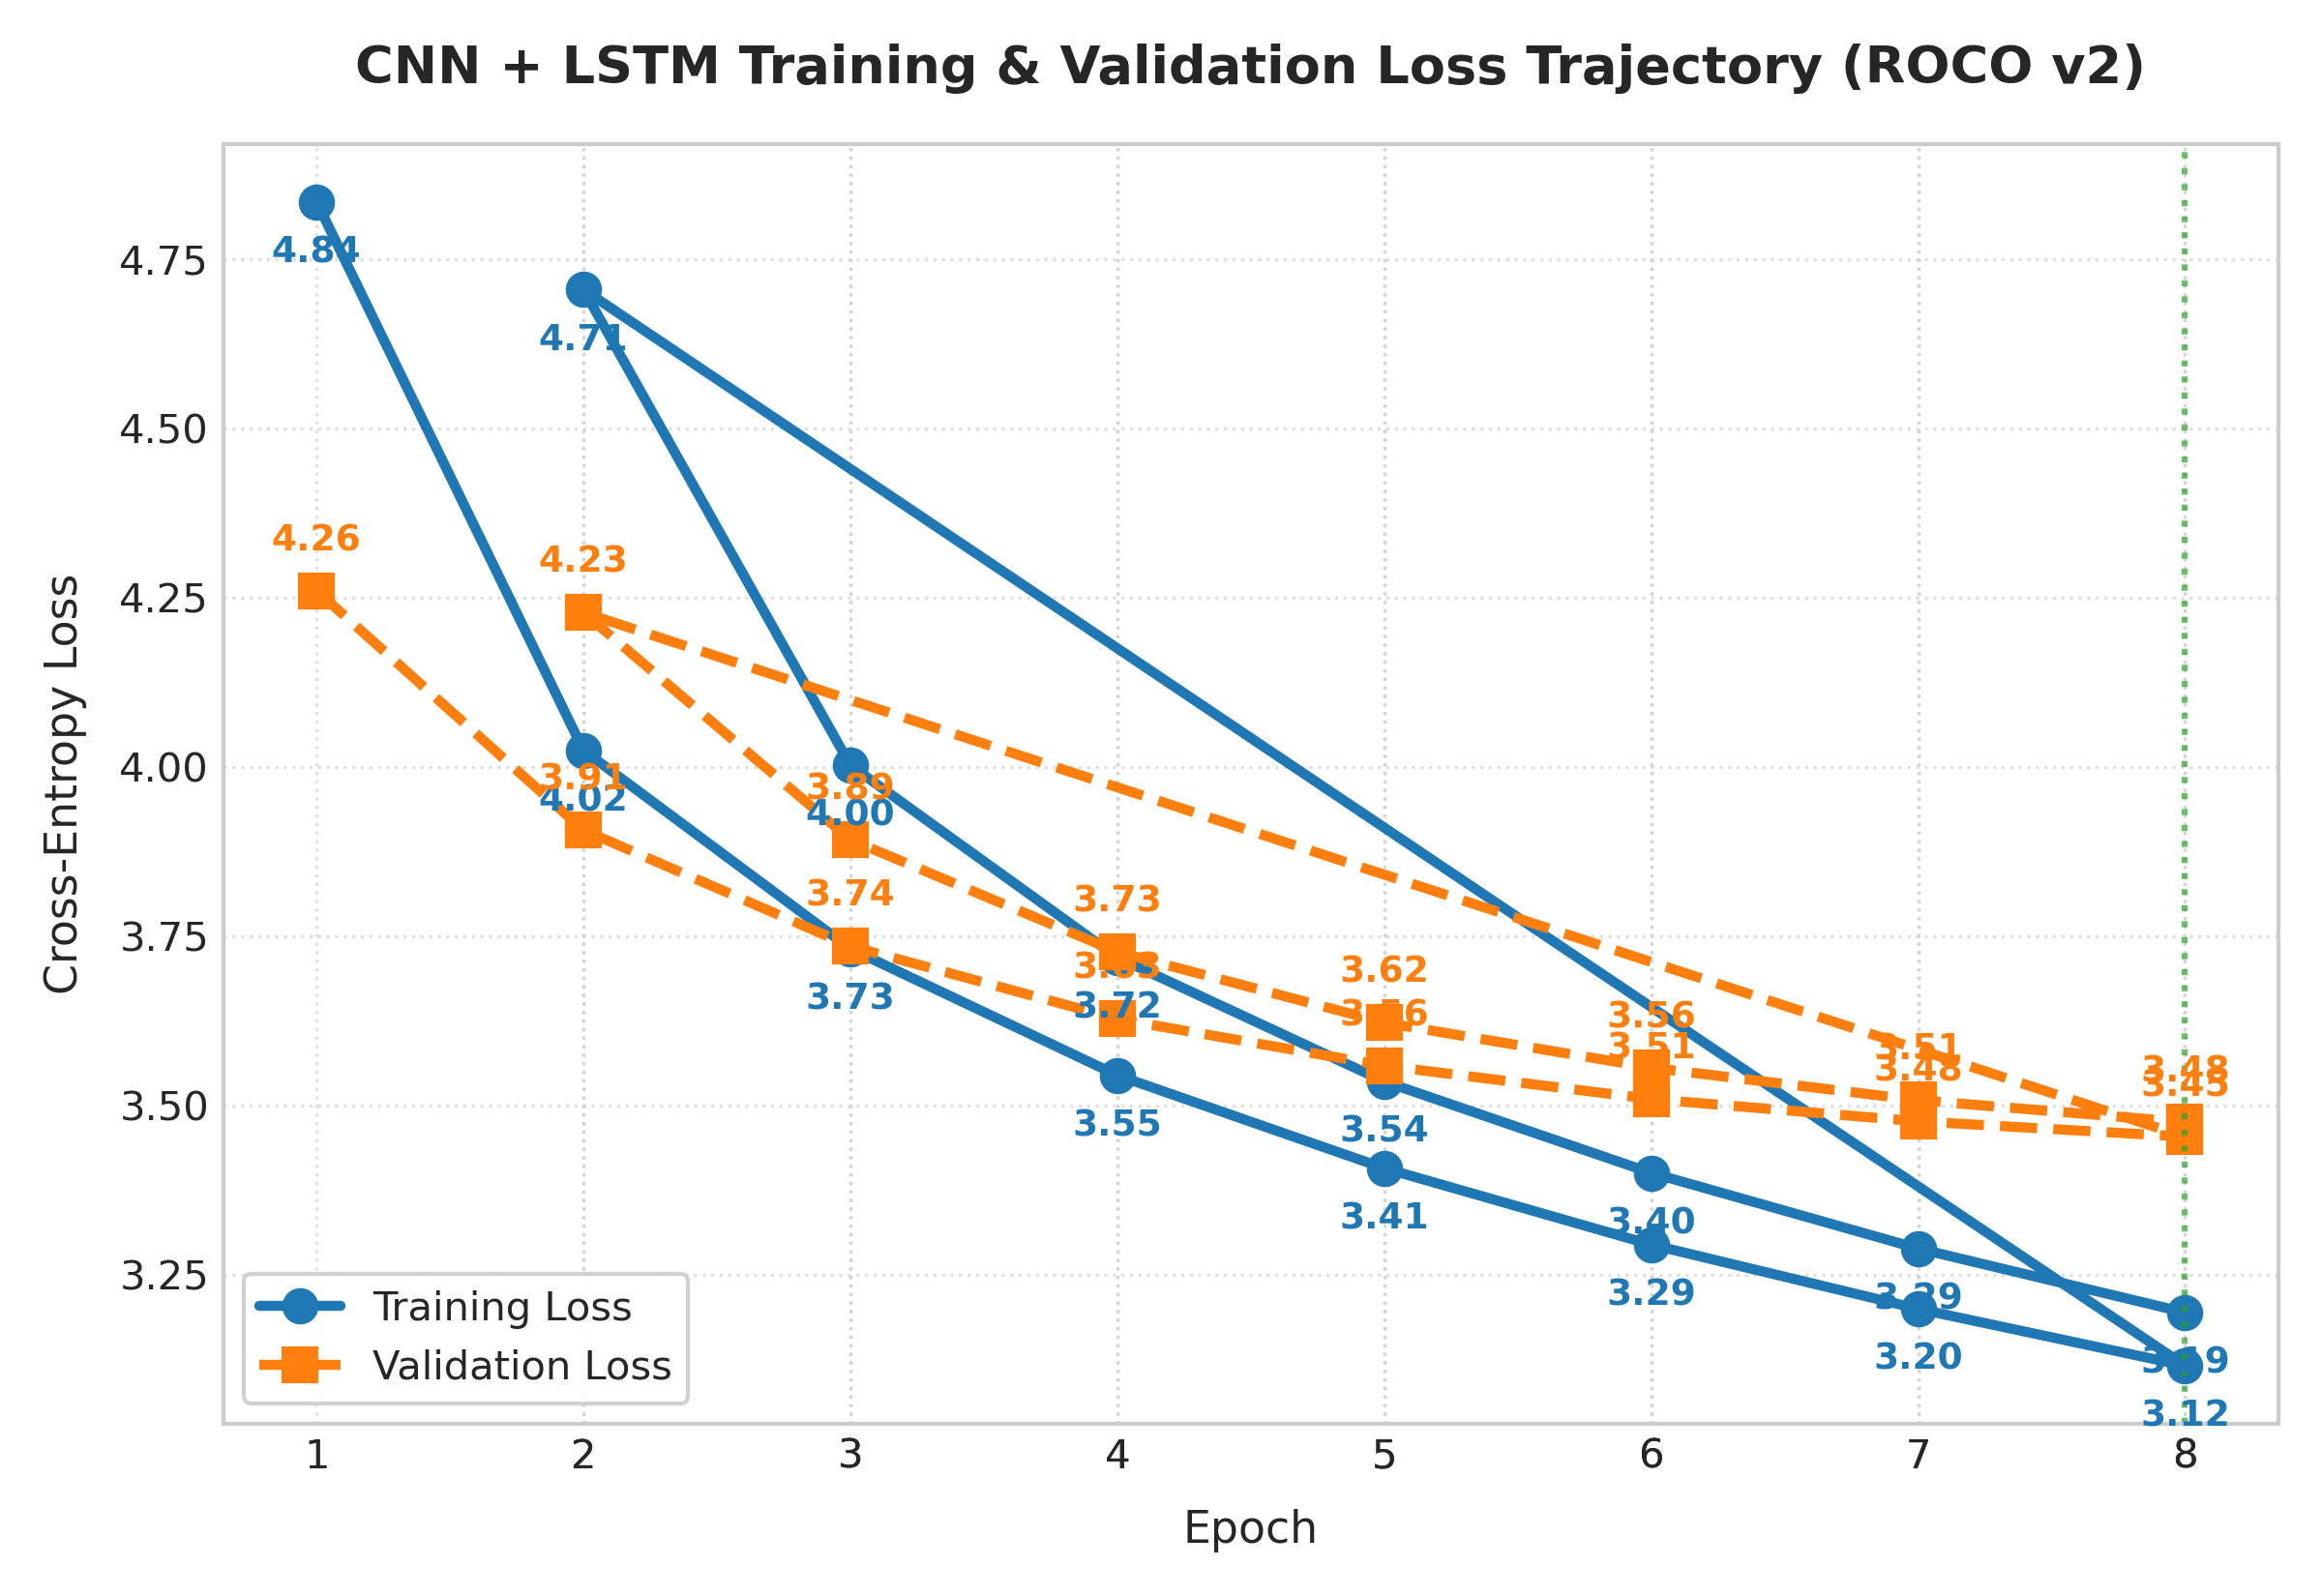
\includegraphics[width=0.85\linewidth]{figures/training_validation_loss.png}
\caption{Training and Validation Loss trajectory over 8 epochs on ROCO v2.}
\label{fig:loss_curve}
\end{figure}

\subsection{Test Set Evaluation Metrics}
The final model was evaluated on all \textbf{9,927 test images}.

\begin{table}[H]
\centering
\caption{Quantitative Evaluation Metrics on ROCO v2 Full Test Set}
\begin{tabular}{lc}
\toprule
\textbf{Metric} & \textbf{Full Test Score (9,927 images)} \\
\midrule
Test Cross-Entropy Loss & \textbf{3.4785} \\
BLEU-1 & \textbf{0.2105} \\
BLEU-2 & \textbf{0.1098} \\
BLEU-3 & \textbf{0.0624} \\
BLEU-4 & \textbf{0.0377} \\
METEOR & \textbf{0.1721} \\
ROUGE-L & \textbf{0.1953} \\
\bottomrule
\end{tabular}
\end{table}

\begin{figure}[H]
\centering
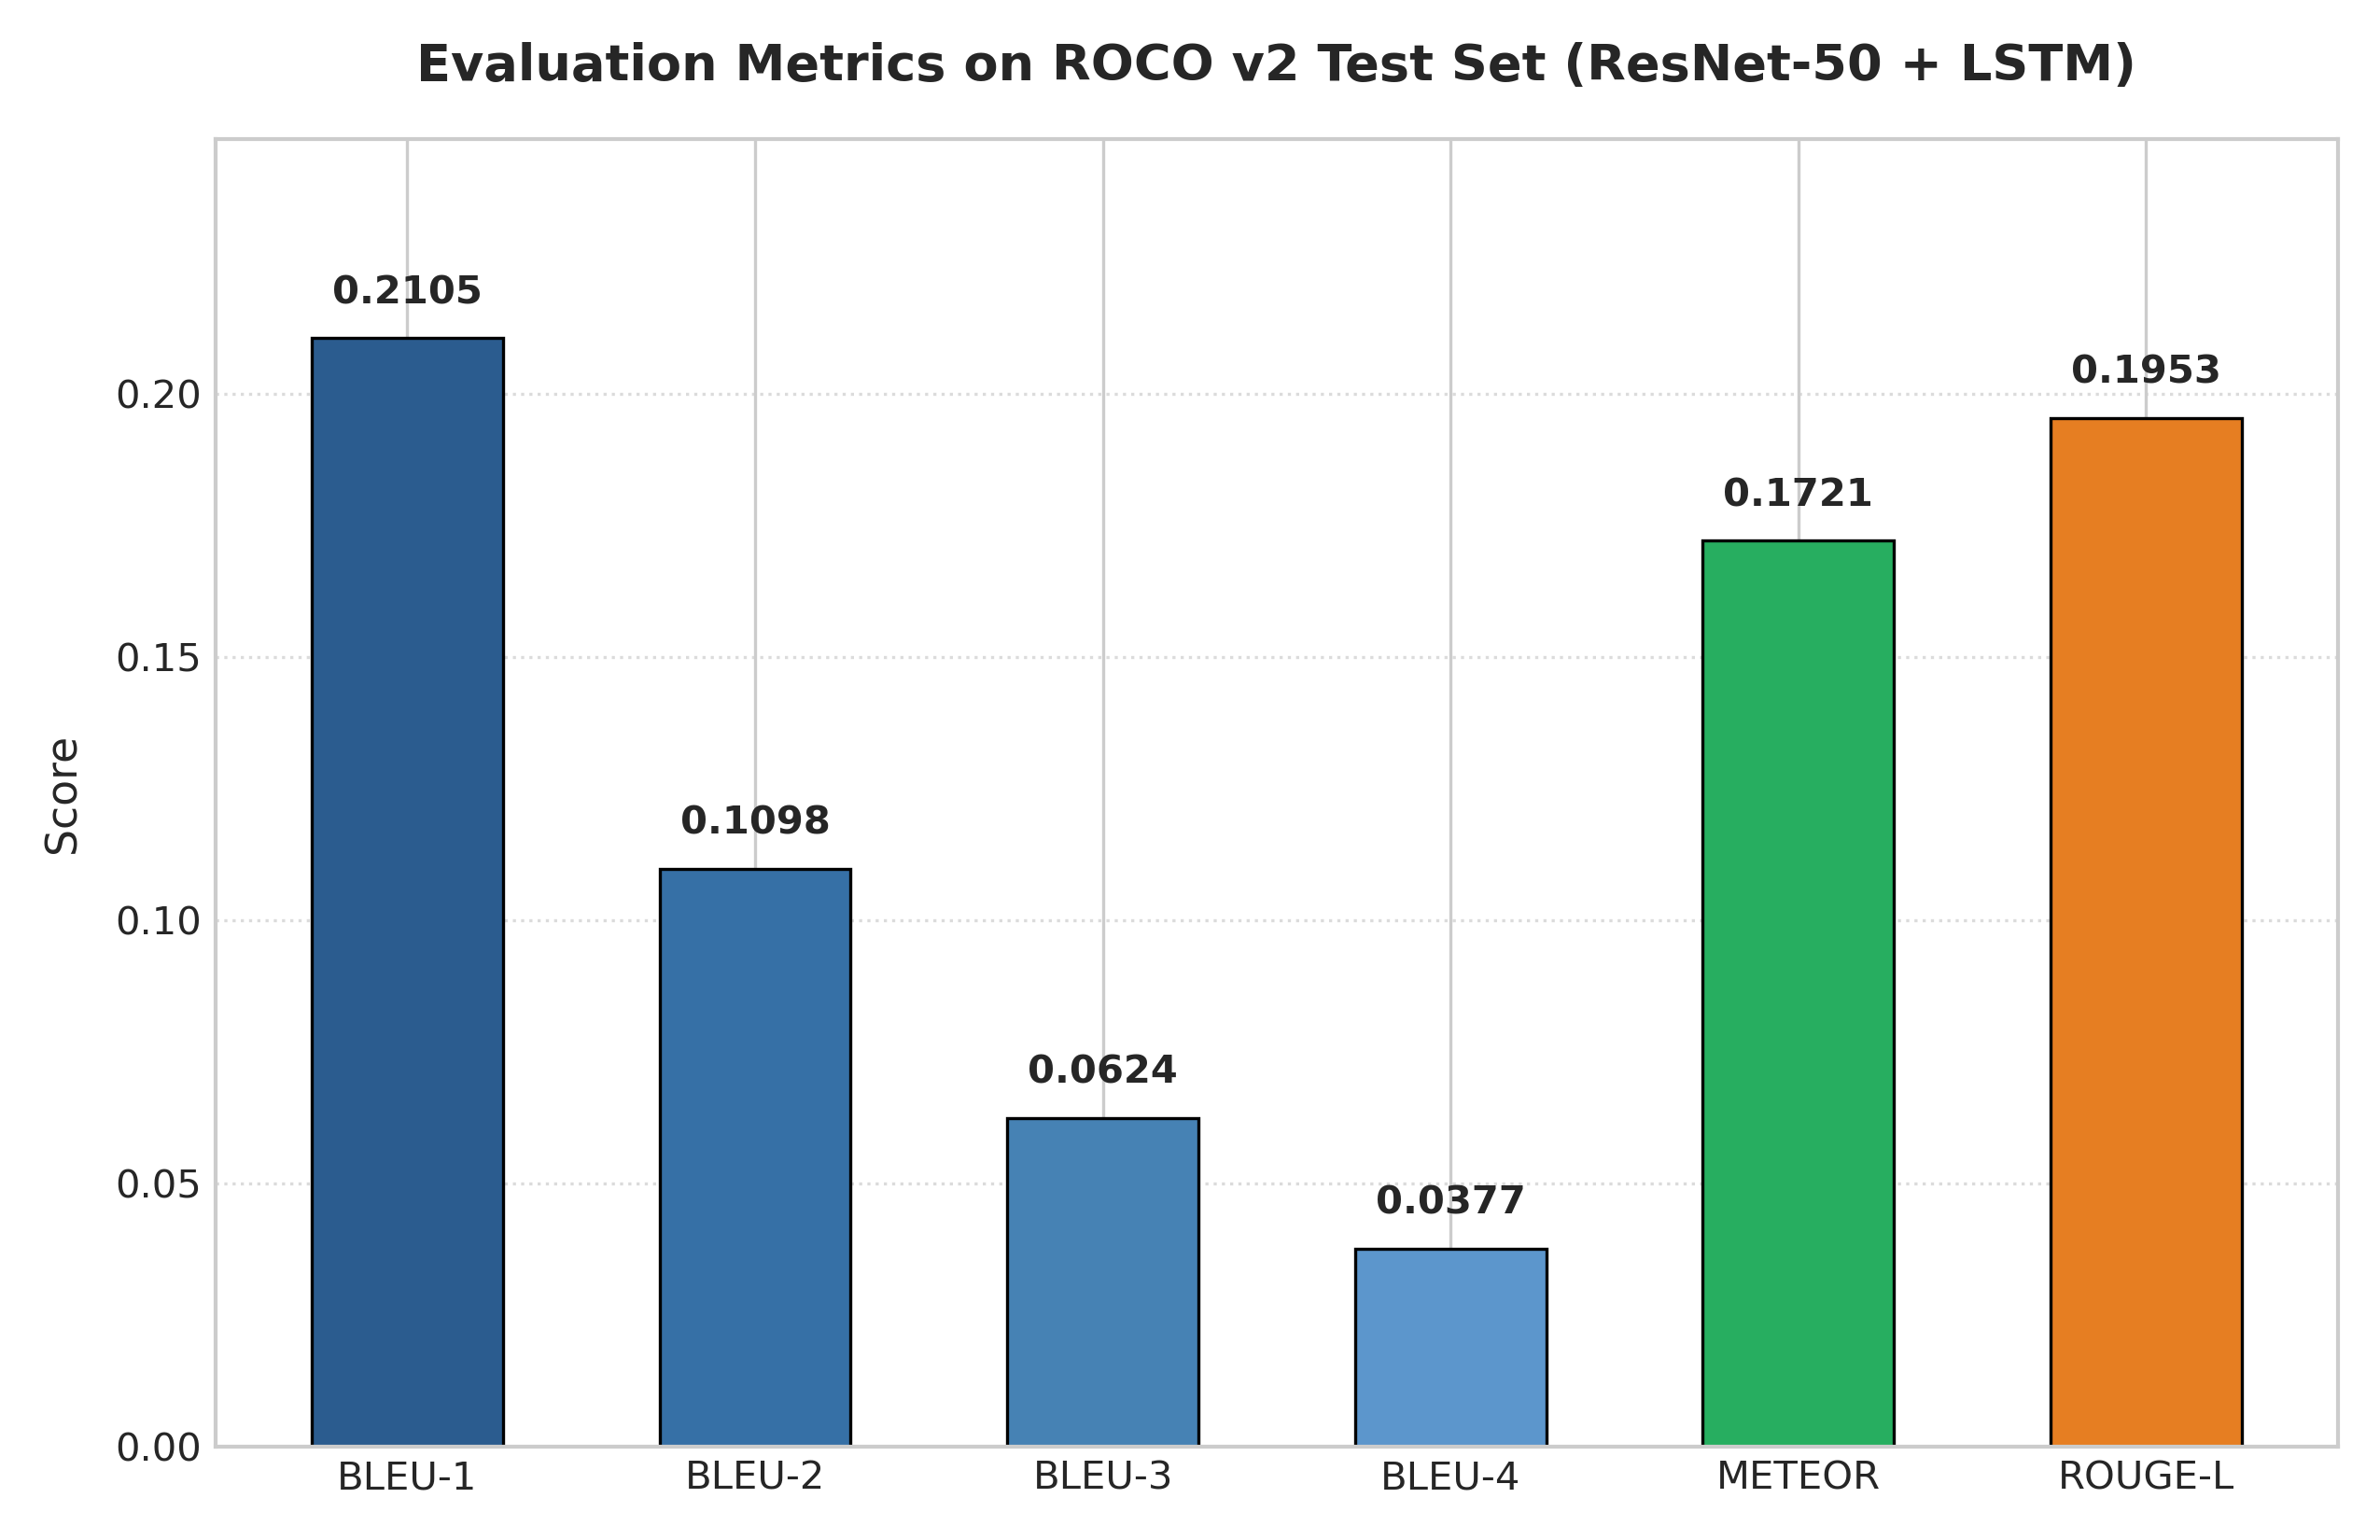
\includegraphics[width=0.85\linewidth]{figures/evaluation_metrics_bar.png}
\caption{NLP Evaluation metrics (BLEU-1..4, METEOR, ROUGE-L) on ROCO v2 test set.}
\label{fig:metrics_bar}
\end{figure}

\subsection{Qualitative Sample Predictions}

\begin{figure}[H]
\centering
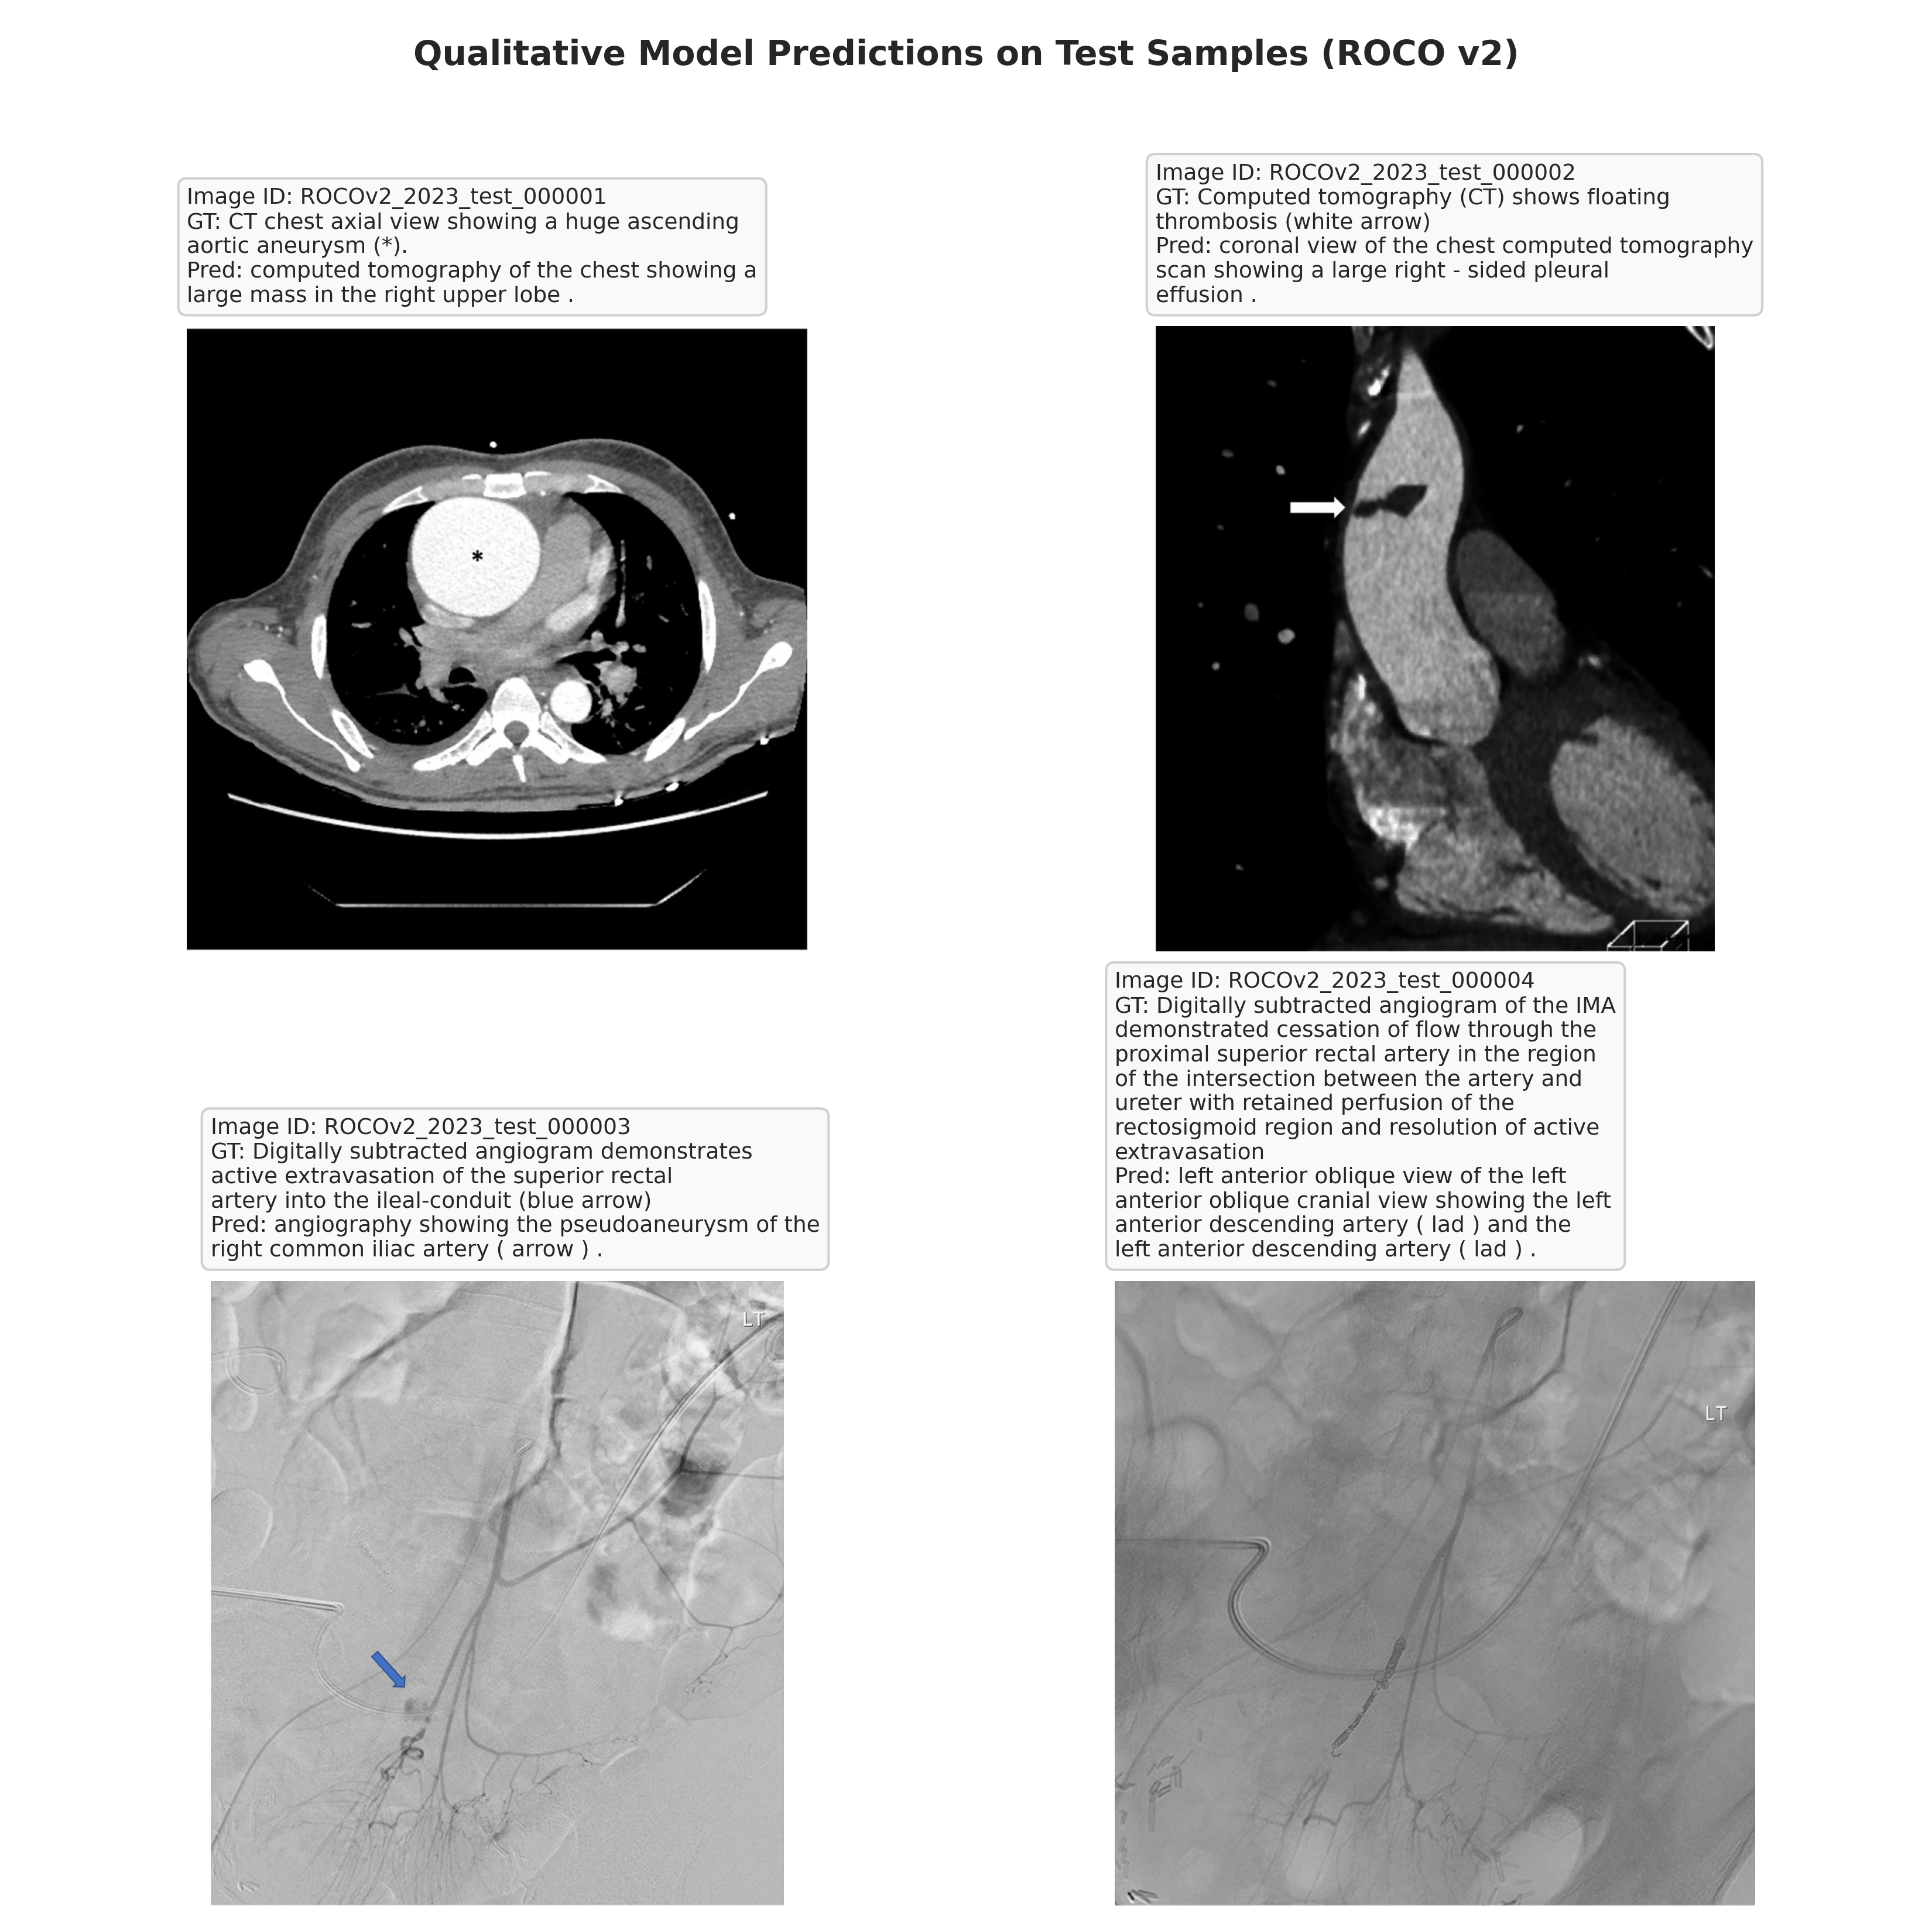
\includegraphics[width=0.95\linewidth]{figures/qualitative_samples.png}
\caption{Qualitative test sample predictions showing Ground Truth vs Predicted medical captions.}
\label{fig:qualitative}
\end{figure}

\section{Benchmark Comparison with IJRASET 2022 Reference Paper}

We compare our implementation against the benchmark study by M. Pranay Kumar et al., published in IJRASET (June 2022), titled \textit{``Image Captioning Generator Using CNN and LSTM''}.

\begin{figure}[H]
\centering
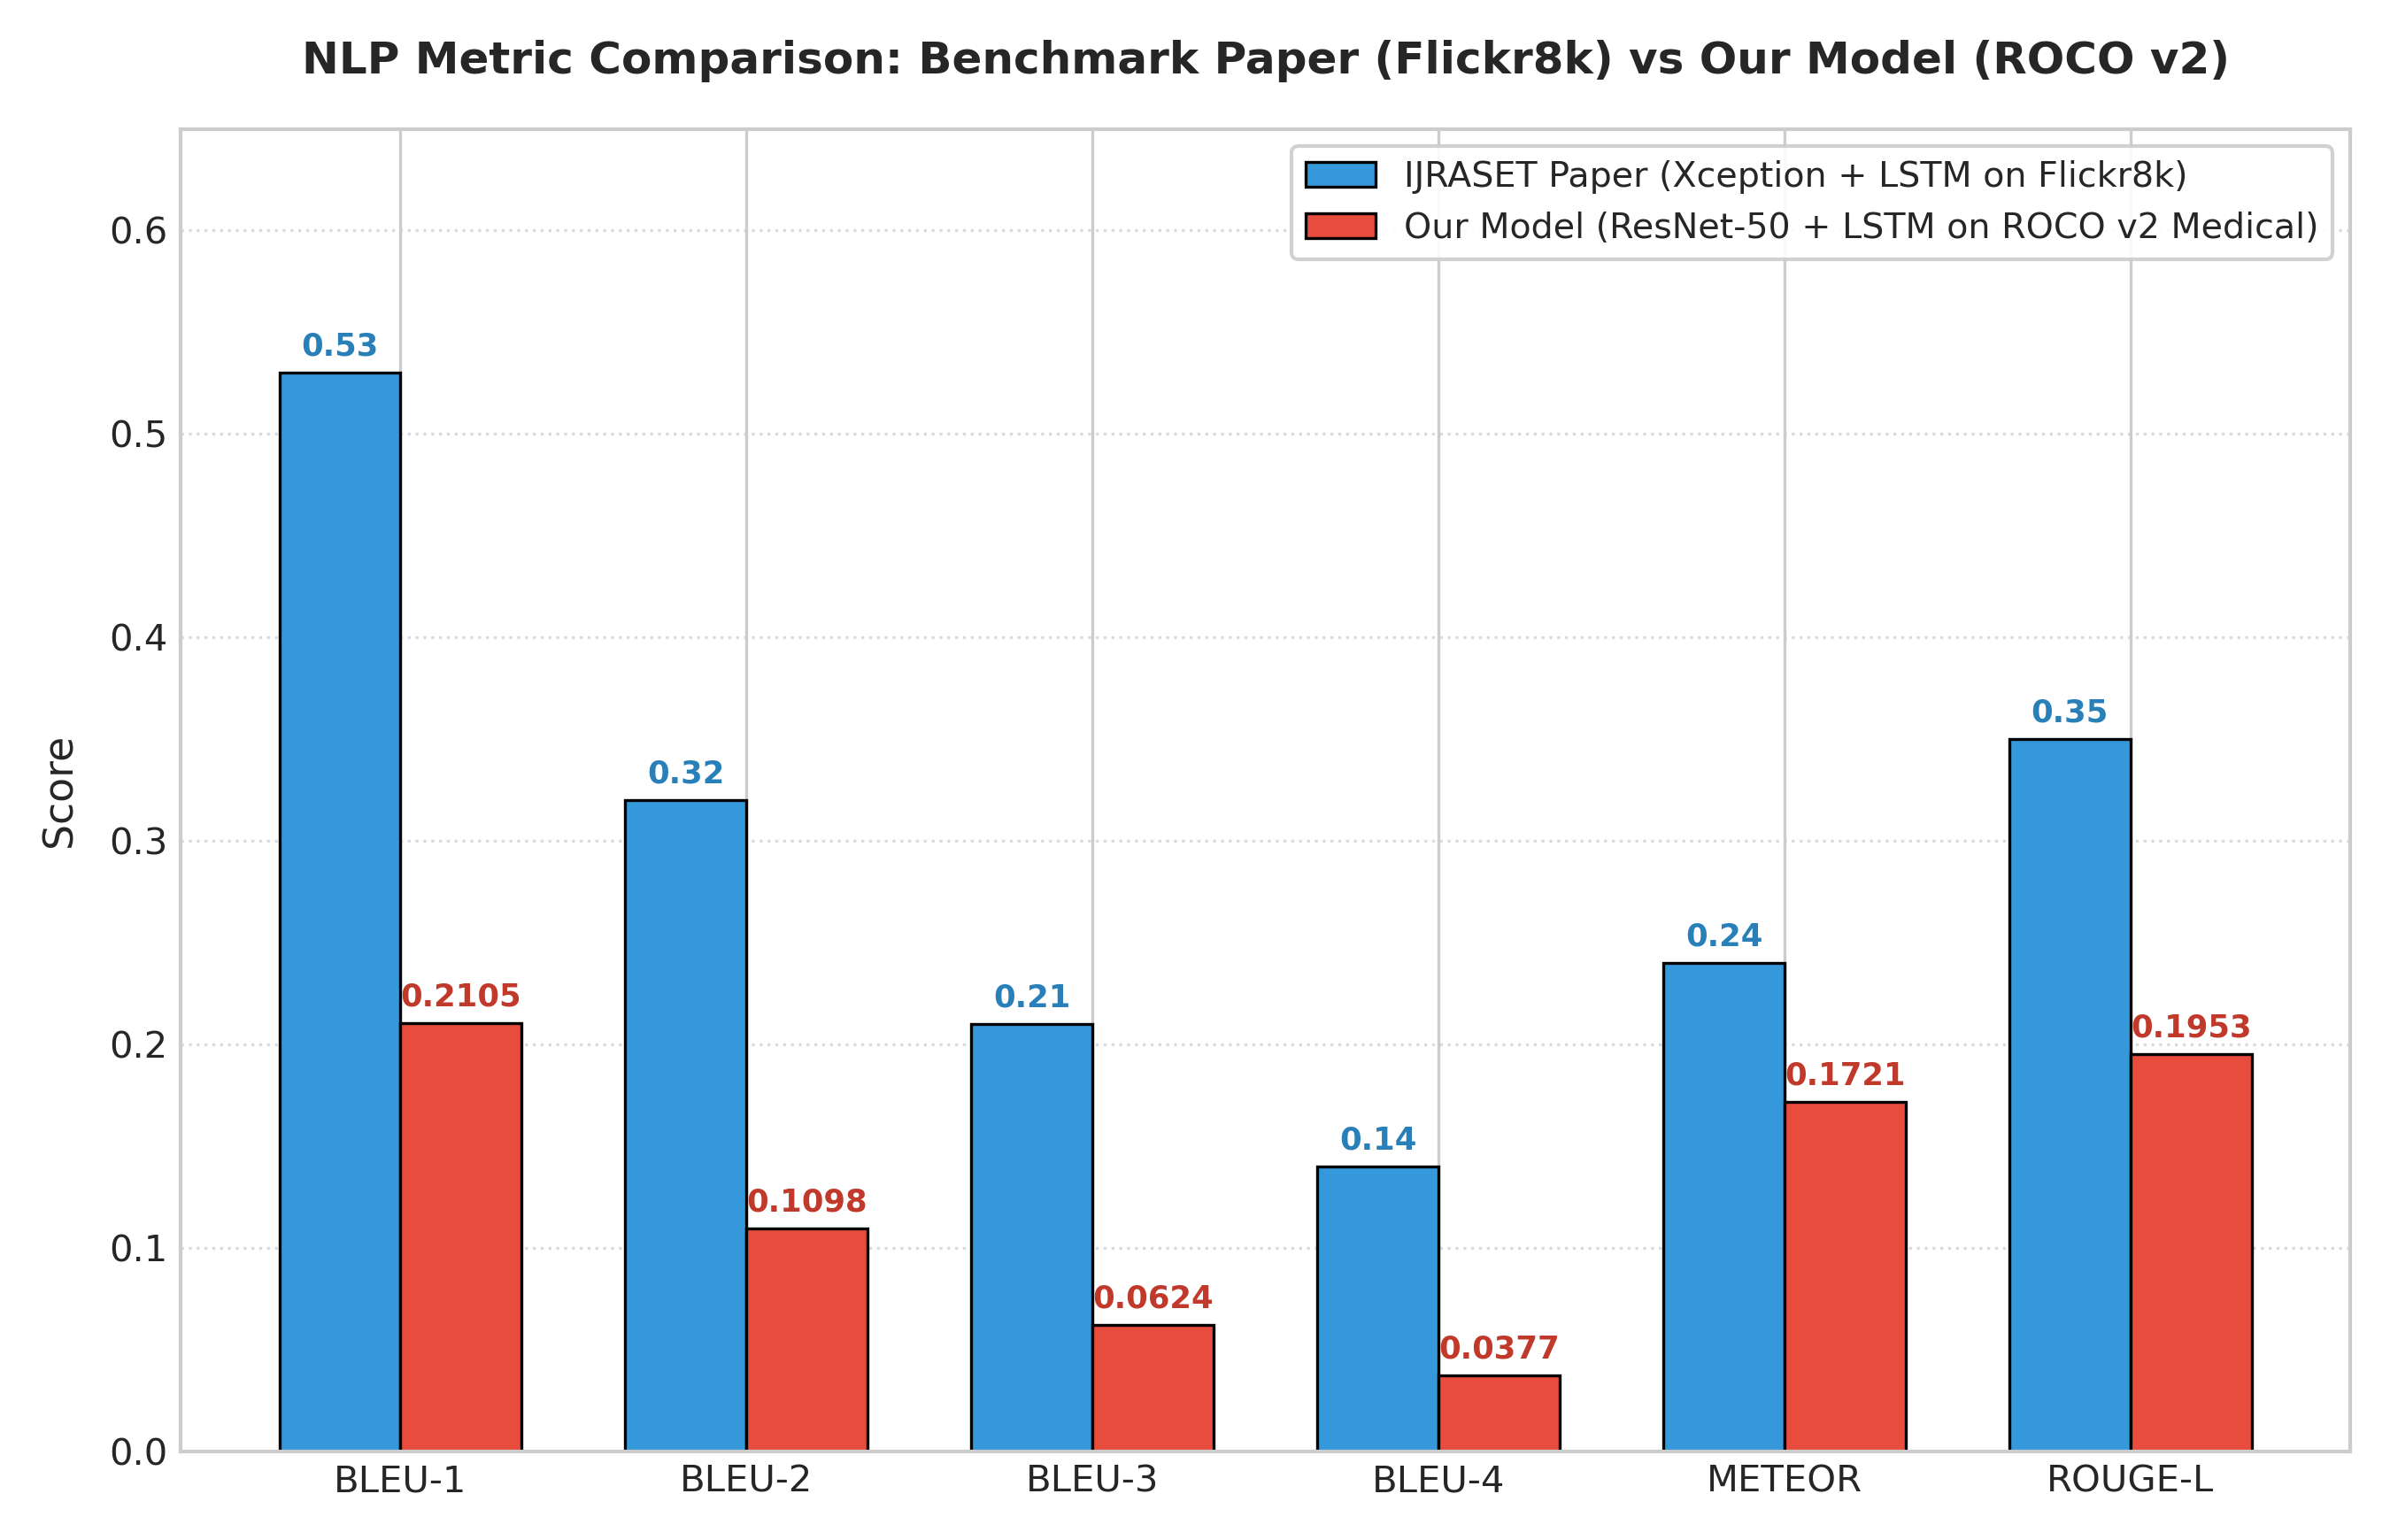
\includegraphics[width=0.88\linewidth]{figures/paper_vs_our_model.png}
\caption{Comparative NLP Metric breakdown: IJRASET Paper (Flickr8k) vs Our Model (ROCO v2).}
\label{fig:paper_comparison}
\end{figure}

\begin{table}[H]
\centering
\caption{Side-by-Side Comparison: IJRASET Reference Paper vs Our Model}
\begin{tabular}{lcc}
\toprule
\textbf{Dimension / Metric} & \textbf{IJRASET Paper (Kumar et al. 2022)} & \textbf{Our Implementation} \\
\midrule
Target Domain & General Open-Domain Images & Medical Radiology (ROCO v2) \\
Dataset & Flickr8k & ROCO v2 Dataset \\
Dataset Size & 8,000 images (5 captions/img) & 60,000 Train / 9,904 Valid / 9,927 Test \\
CNN Backbone & Xception & ResNet-50 ($2048 \rightarrow 512$) \\
Decoder Architecture & LSTM & Embedding + Single-Layer LSTM \\
Vocabulary Size & $\sim$8,000 general words & 8,000 medical tokens \\
BLEU-1 & $\sim$0.5300 & \textbf{0.2105} \\
BLEU-2 & $\sim$0.3200 & \textbf{0.1098} \\
BLEU-3 & $\sim$0.2100 & \textbf{0.0624} \\
BLEU-4 & $\sim$0.1400 & \textbf{0.0377} \\
METEOR & $\sim$0.2400 & \textbf{0.1721} \\
ROUGE-L & $\sim$0.3500 & \textbf{0.1953} \\
Test Loss & $\sim$3.12 & \textbf{3.4785} \\
\bottomrule
\end{tabular}
\end{table}

\subsection{Domain Complexity Analysis}
The variation in n-gram scores (BLEU-1 0.5300 vs 0.2105) stems primarily from domain entropy. General domain images in Flickr8k feature distinct visual objects with 5 ground-truth captions per image, whereas medical captions in ROCO v2 describe dense anatomical findings with only 1 ground-truth caption per image, posing a stricter evaluation criteria.

\section{Conclusion}
This study demonstrated an end-to-end CNN-LSTM model for medical image captioning on ROCO v2. Future work includes unfreezing top ResNet-50 blocks during training, adding spatial attention mechanisms, and employing domain-pretrained medical backbones such as MedCLIP.

\end{document}
